%*****************************************
\chapter{Review of Talbot-Lau interferometry}\label{ch:review}

\section{X-ray interaction with matter}

Immediately after their discovery in 1895, X-rays drew attention from the
medical community for their unprecedented ability of generating an image of
hidden part of a sample. What makes this kind of electromagnetic radiation
particularly useful as a probe is the fact that it interacts with matter
just strongly enough to carry information about the materials it passes
through, yet weakly enough to penetrate the entire volume.

In order to reconstruct some physical properties of a sample through the
observation of its interaction with X-rays, it is possible to introduce a
sequence of approximation to Maxwell's equations in a medium:
\begin{align}
    \nabla \cdot \vec{D} & = \rho \label{eq:gauss}\\
    \nabla \cdot \vec{B} & = 0 \label{eq:nomonopoles}\\
    \nabla \times \vec{E} + \partial_t \vec{B} & = 0
    \label{eq:induction}\\
    \nabla \times \vec{H} - \partial_t \vec{D} & = \vec{J}
    \label{eq:ampere}.
\end{align}

In general, the electric field $\vec{E}$, the magnetic field $\vec{H}$, the
electric displacement field $\vec{D}$ and the magnetic induction field
$\vec{B}$, the charge density $\rho$ and the current density $\vec{J}$ are
functions of the three spatial coordinates and time. 

However, a number of restrictions and approximations can be introduced to
simplify the equations. We are indeed interested in the case where there are
no charge or current sources

\begin{equation}
    \rho = 0\\
    \vec{J} = 0.
    \label{eq:absentsources}
\end{equation}

It follows that the electric and magnetic fields can be decoupled, since
taking the curl of~\eqref{eq:induction} yields

\begin{equation}
    \nabla \times (\nabla \times \vec{E}) + \partial_t(\nabla \cdot \vec{B}) = 0,
    \label{}
\end{equation}
where the second summand is zero by equation~\eqref{eq:nomonopoles}:

\begin{align}
    \nabla \times (\nabla \times \vec{E}) &= 0\\
    \nabla^2 \vec{E} - \nabla (\nabla \cdot \vec{E}) = 0.
    \label{}
\end{align}

Similarly, the electric field can be eliminated from
equation~\eqref{eq:ampere} by taking the curl and substituting
equation~\eqref{eq:gauss}.

We further restrict the materials to be isotropic and linear, that is
$\vec{D}(t, \vec{x}) = \varepsilon(\vec{x}) \vec{E}(t, \vec{x})$, where the
electric permeability coefficient is also independent of time. Moreover, we
exclude magnetic materials by setting $\vec{B} = \mu_0 \vec{H}$.

\begin{align*}
    \left(\varepsilon \mu_0 \partial^2_t - \nabla^2 \right)
    \vec{E} &= - \nabla(\nabla \cdot \vec{E}) \\
    \left(\varepsilon \mu_0 \partial^2_t - \nabla^2 \right)
    \vec{H} &= \frac{1}{\varepsilon}\nabla \varepsilon \times (\nabla \times
    \vec{H}).\\
\end{align*}

These two equations do not couple the magnetic and the electric field, but
they still mix different cartesian components of each components of each
field through their second derivatives. If the electron density varies slowly
with respect to the wavelength of the X-rays, we can neglect such mixed
derivative terms, and obtain a scalar equation for each cartesian component
of the electric field

\begin{equation}
    \left( \varepsilon(\vec{x}) \mu_0 \frac{\partial^2}{\partial t^2} - \nabla^2
    \right) \hat{\psi}(t, \vec{x}) = 0.\label{eq:helmoltz.spacetime}
\end{equation}

This equation, known as the Helmoltz equation is better understood when
taking the Fourier transform with respect to time:

\begin{equation*}
    \hat{\psi}(t, \vec{x}) =
    \frac{1}{\sqrt{2\pi}}\int_{0}^{\infty}\psi(\omega, \vec{x})
    e^{-i \omega t} \de{\omega}.
\end{equation*}

The time derivative becomes then $\partial_t = - i\omega = -i c k$, and the
equation can be finally written as

\begin{equation*}
    \left( \varepsilon_\omega(\vec{x}) \mu_0 c^2 k^2 + \nabla^2
    \right) \psi(\omega, \vec{x}) = 0.
\end{equation*}

Or, introducing the refractive index $n_\omega =
c\sqrt{\varepsilon_\omega\mu_0}$:

\begin{equation}
    \left( n_\omega^2(\vec{x}) k^2 + \nabla^2
    \right) \psi(\omega, \vec{x}) = 0.\label{eq:helmoltz.fourier}
\end{equation}

The fact that the interaction of X-rays with matter is both strong enough to
be a meaningful probe of physical properties and weak enough to penetrate an
entire macroscopical can be precisely expressed by the following
\emph{ansatz} to the solution of equation~\eqref{eq:helmoltz.fourier}:
    \begin{equation*}
 \psi(\omega, x, y, z) = \tilde{\psi}(\omega, x, y, z) \exp(ikz),    
\end{equation*}
that is, the solution is a product of a freely propagating plane wave
$\exp(ikz)$ and of a perturbation $\tilde{\psi}$ introduced by the sample.

With  $\nabla_\perp^2 = \partial_x^2 + \partial_y^2$, the Helmoltz
equation~\eqref{eq:helmoltz.fourier} becomes
\begin{equation*}
    \left[ 2ik \frac{\partial}{\partial z} + \nabla_\perp^2 +
    \frac{\partial^2}{\partial z ^2} + k^2 (n^2_\omega(\vec{x}) - 1)
\right]\tilde{\psi}(\omega, \vec{x}) = 0,
\end{equation*}
where the \emph{weak} interactions allow us to introduce the paraxial
approximation, where the variations along the $z$ axis, expressed by the
second derivative $\partial_z^2$ are negligible with
respect to the perpendicular $x-y$ plane. Moreover, the terms with
$\nabla_\perp^2$ can also be neglected as they are responsible of coupling
neighbouring X-ray trajectories.

Finally we can write the equation for the amplitude of the perturbation introduced by a
sample in the X-ray beam as
\begin{equation}
    \partial_z \tilde{\psi}(\omega, x, y, z) =
    \frac{k}{2i}(1 - n^2_\omega(\vec{x}))\tilde{\psi}(\omega, x, y, z).
    \label{eq:helmoltz.perturbation}
\end{equation}

The complex number $n_\omega$ is the refractive index, it is usually
very close to 1 in this energy range, and the imaginary and real parts are
usually explicitly considered:

\begin{equation*}
    n_\omega = 1 - \delta_\omega + i\beta_\omega.
\end{equation*}

Since both $\delta \ll 1$ and $\beta \ll 1$ the terms of order $\beta^2$ and
$\delta^2$ can be neglected in equation~\eqref{eq:helmoltz.perturbation}.
The solution is then easily found by integrating with respect to $z$
(figure~\ref{fig:propagation})

\begin{figure}[htb]
    \centering
    \input{gfx/interaction.eepic}
    \caption[Plane wave propagation.]{A plane wave propagates along the $z$
        axis through an object from $z = 0$ to $z = z_0$.}
    \label{fig:propagation}
\end{figure}

\begin{equation}
    \tilde{\psi}(\omega, x, y, z_0) = \exp\left\{-ik\int_{z=0}^{z=z_0}(\delta_\omega - i
\beta_\omega) \de z \right\} \tilde{\psi}(\omega, x, y, 0),
\label{eq:helmoltz.solution}
\end{equation}
where the effects of the sample perturbations can be described as the sum of
a phase shift determined by the real part of the refractive index $\delta$
\begin{equation*}
    \Delta\varphi(x, y) = -k \int \delta_\omega(x, y, z) \de z
    %\label{eq:phase_deviation}
\end{equation*}
and an attenuation of the intensity, that is the square modulus of the
amplitude $I = |\psi|^2$, according to the Beer-Lambert law
\begin{equation}
    I(\omega, x, y, z_0) = \exp\left\{-2k\int \beta_\omega(x, y, z) \de
    z\right\}
    I(\omega, x, y, 0).\label{eq:beer-lambert}
\end{equation}

We can then conclude that the interaction of X-rays with a sample, that is
with the electron clouds of the atoms that make it up, is determined by
two energy-dependent coefficients $\delta$ and $\beta$. These have been
thoroughly studied and tabulated\cn{NIST database} through the atomic form
factors $f_1$ and $f_2$ respectively. The relationship between the
refractive index, $delta$, $beta$ and the atomic form factors $f_1$ and
$f_2$ that is used to calculate the expected theoretical values in this
thesis is:

\begin{equation}
    n = 1 - \delta + i\beta = 1 - \frac{r_e\lambda^2}{2\pi}(f_1 + if_2).
    \label{eq:atom.factors}
\end{equation}

Far from absorption edges, these coefficients depend on the atomic number
$Z$ roughly as

\begin{align}
    \beta &\propto Z^3 / k^4
    \delta &\propto Z / k^2.
    \label{eq:delta.beta.energy}
\end{align}

This leads to the conclusion that the phase term $\delta$ becomes
relatively more important as the energy of the beam and the atomic number
are increased~(see figure~\ref{fig:delta.beta}).

\begin{figure}[htb]
    \centering
    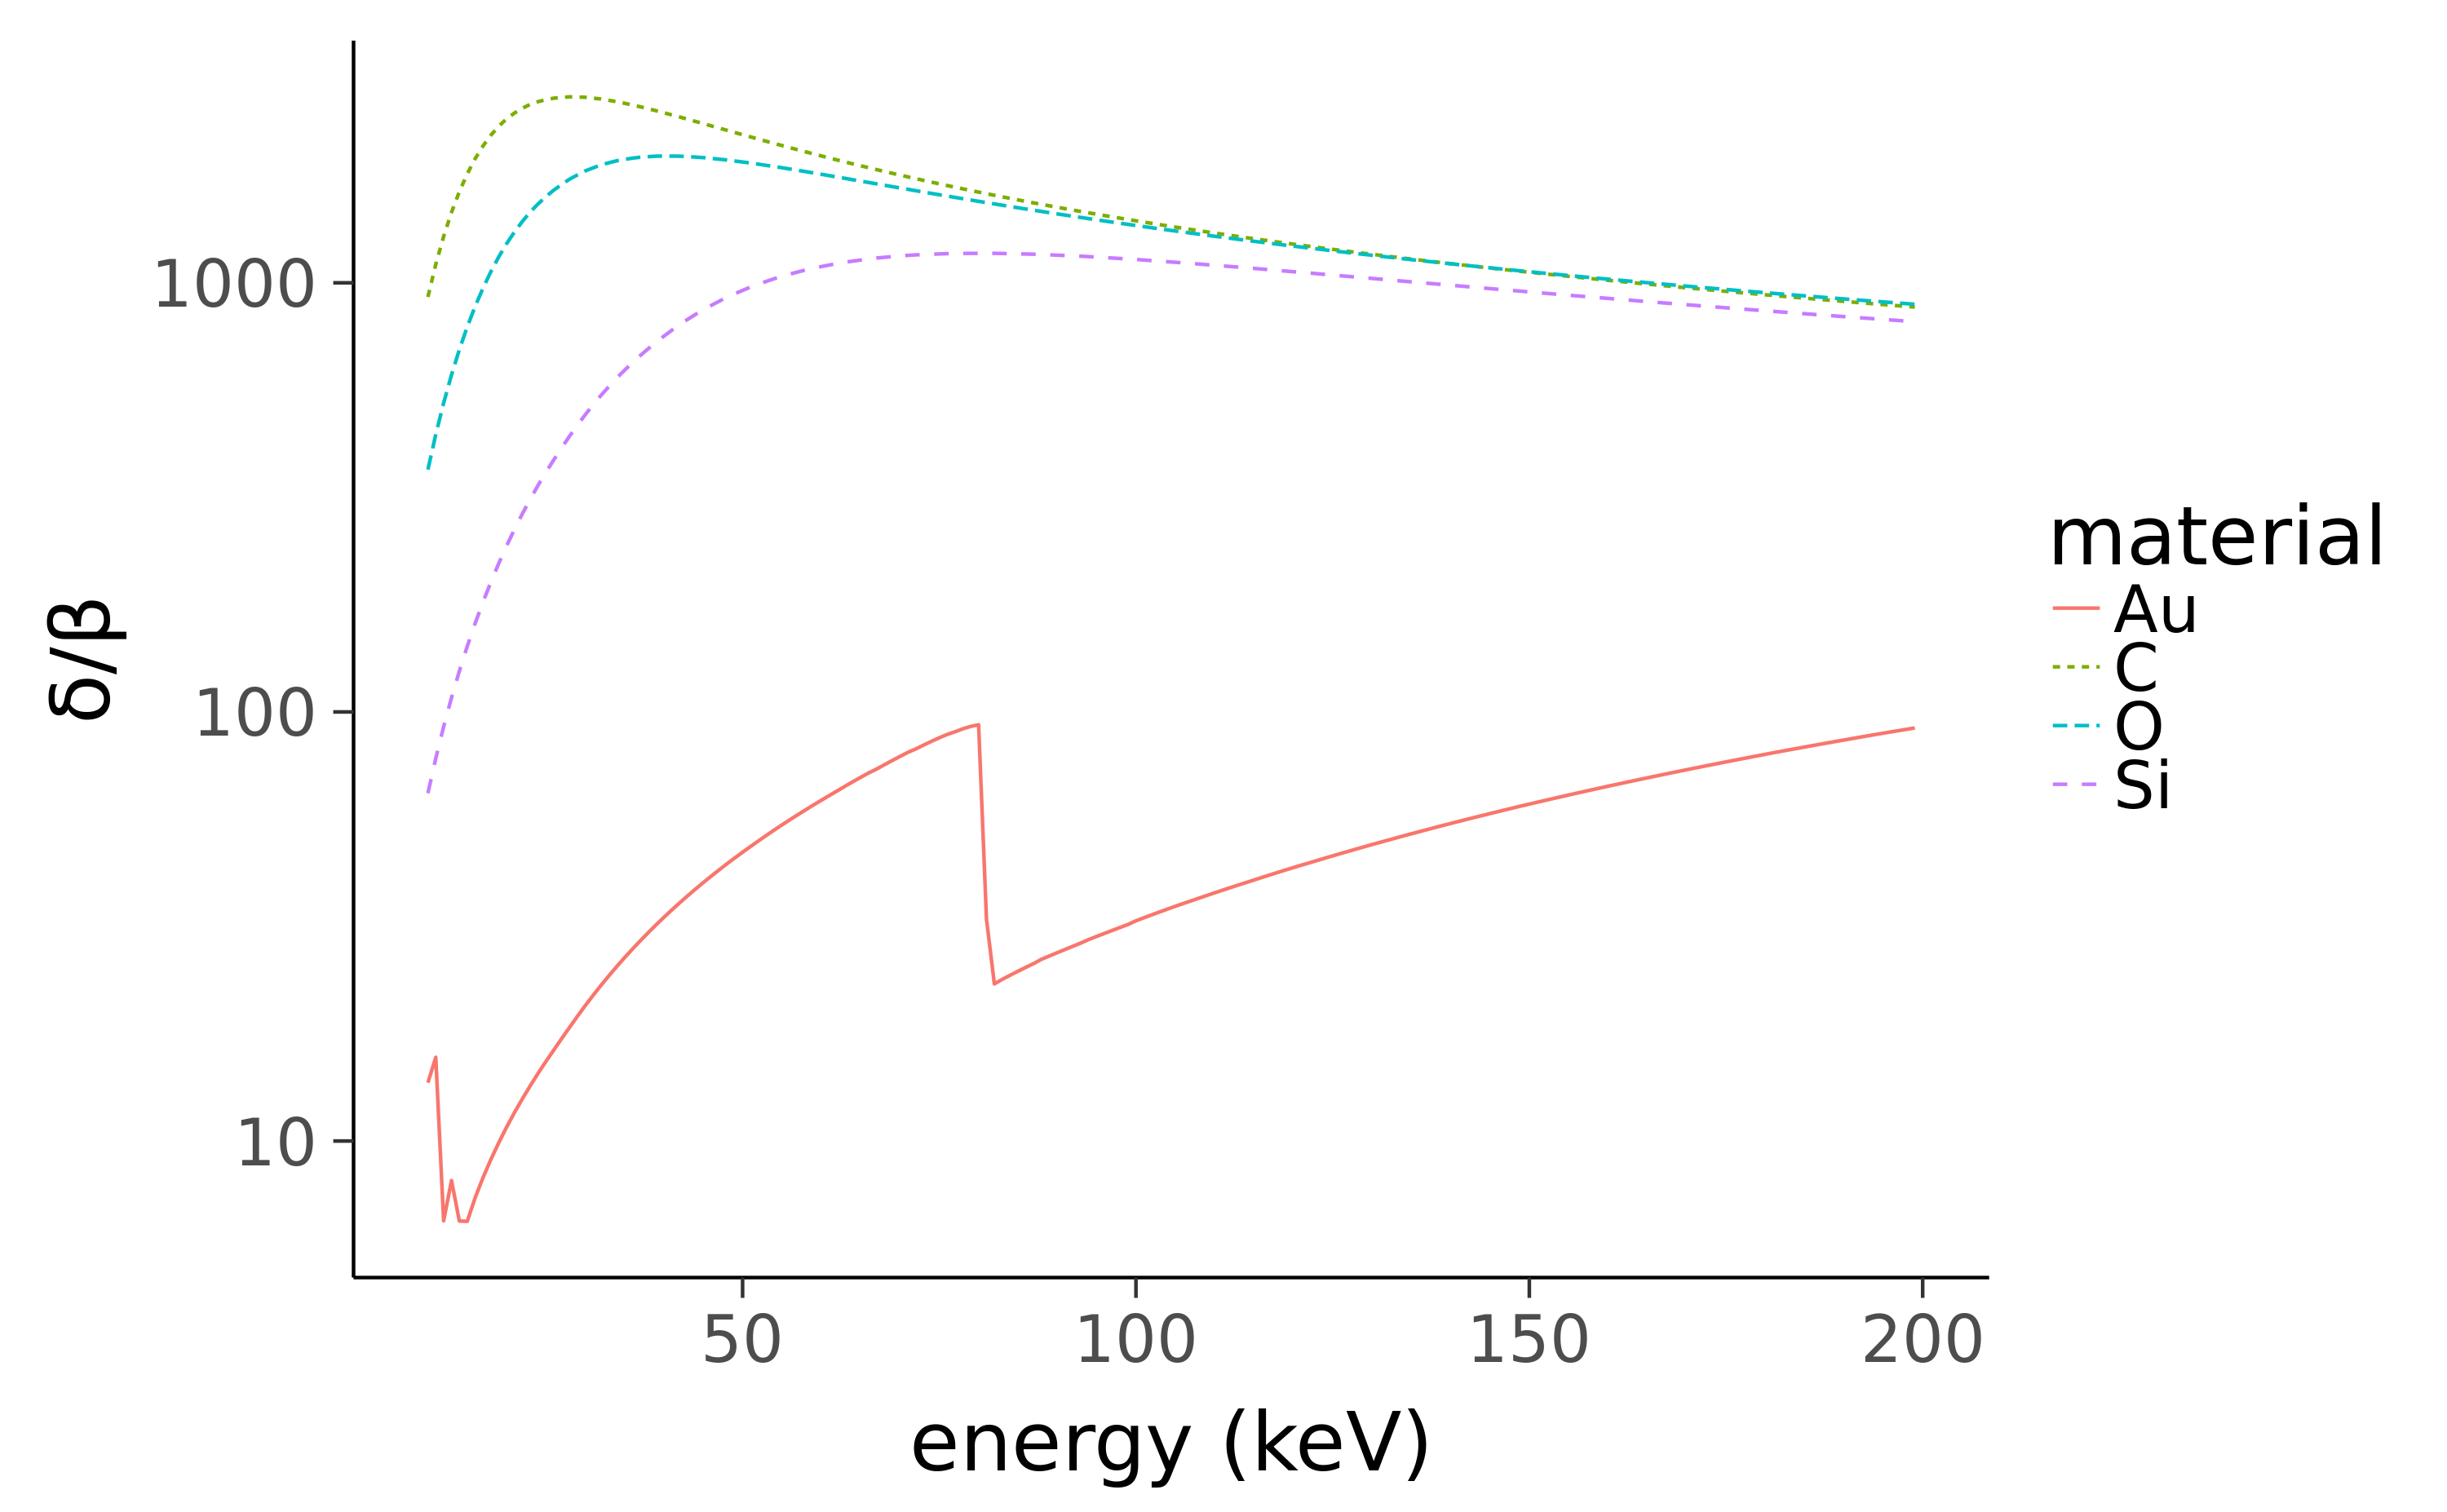
\includegraphics[width=\textwidth]{gfx/delta-beta-comparison/delta-beta-comparison.png}
    \caption[Values of $\delta/\beta$ as a function of energy for different
    materials.]{Ratio of $\delta$ to $\beta$. $\delta$ contributes to the
    phase interaction, while $\beta$ is the term for absorption in the
refractive index. The ratio shows that the phase interaction is stronger
than absorption interaction and that it also becomes relatively stronger as
the energy increases up to stabilizing at a value that is larger for
materials with a higher atomic number.}
    \label{fig:delta.beta}
\end{figure}


A voltage of 60 to \SI{140}{\kilo\voltpeak} is commonly used for medical and
security applications, or even higher for material sciences for the
inspection of large volumes or materials with a high atomic number.
Phase-contrast with grating interferometers has seen so far only limited
applications\cn to a lower energy range.
This is the fundamental motivation of this experimental work, in order to
assess the feasibility and characteristics of X-ray interferometric
techniques for standard laboratory sources with a higher beam energy.

\section{Interferometry}

The results of the previous sections, and in particular,
equation~\eqref{eq:helmoltz.solution} point to the possibility of recovering
additional information on a sample through the knowledge of the real part of
the refractive index $\delta$. Unfortunately, only the intensity $I =
|\psi|^2$ of the X-ray beam can be directly detected, and an interferometric
setup is needed to convert phase differences into intensity modulations.
Various approaches have been presented in the last decades, on different
applications and source types. The main methods are summarized in the
following sections, with a detailed description of Talbot-Lau interferometry
which will be our weapon of choice.

\subsection{Propagation-based phase contrast}
Techniques based on free-space propagation of X-rays have been widely
explored on both monochromatic and polychromatic sources. If a weakly
absorbing object si placed at a distance $R_1$ from a coherent X-ray source,
it will introduce phase differences whose laplacian can be observed as an
intensity modulation at a distance $R_2$ downstream (figure~\ref{fig:propagation.based}), with
$M = (R_1 + R_2) / R_1$ as the geometrical magnification:
\begin{equation}
    I(x, y) = \frac{I_0}{M^2}\left(1 + \frac{R_2\lambda}{2\pi M^2}\nabla_\perp^2
    \varphi(x, y)\right).
    \label{eq:free.space.propagation}
\end{equation}

\begin{figure}[htb]
    \centering
    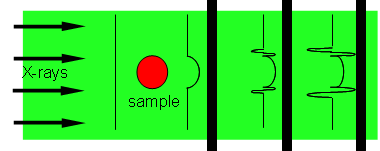
\includegraphics[width=\textwidth]{gfx/propagation-based_imaging.png}
    \caption[Propagation-based setup.]{A propagation-based phase contrast
    setup\cn. The intensity modulations producing edge-enhancing effects can
be observed at different distances in order to reconstruct the phase
differences introduced by the sample according to
equation~\eqref{eq:free.space.propagation}.}
    \label{fig:propagation.based}
\end{figure}

In general, this technique requires recording such diffraction patterns at
multiple distances $R_2$ from the sample in order to unambiguously
reconstruct the phase and therefore the electron density of the sample.
Moreover, a high spatial coherence of the beam is required, which means
that the source must be very small or placed at a large distance $R_1$ from
the sample. The detector also needs to have a high spatial resolution in
order to resolve the intensity modulations of
equation~\eqref{eq:free.space.propagation}. All of these constraints tend to
have a negative impact on exposure times, but a number of applications are
possible, including tomographic imaging and even \emph{in vivo} imaging.

\subsection{Diffraction enhanced imaging}
Diffraction enhanced --- or crystal-based --- methods employ two crystals:
one after the source, to obtain a monochromatic and collimated X-ray beam;
one before the detector, acting as an extremely sensitive angular filter.

The intensity on the detector is modulated by changing the incidence angle
$\vartheta$ of the beam on the second crystal (figure~\ref{fig:dei}).
\begin{figure}[htb]
    \centering
    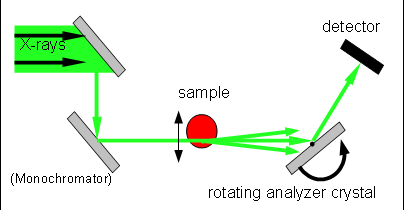
\includegraphics[width=\textwidth]{gfx/analyzer-based_imaging.png}
    \caption[Analyzer-based setup.]{A setup for diffraction enhanced
        imaging\cn. The fine angular deviations introduced in the
    monochromatic beam are decoded through rotations of the analyzer crystal.}
    \label{fig:dei}
\end{figure}
The intensity in each pixel is then recorded through multiple exposures as a
function of $\vartheta$, producing a \emph{rocking curve}. These rocking
curves are sensitive to refraction in a direction perpendicular to the beam
and to the axis of rotation of the analyzer grating, and can provide a
differential phase image, as well as a scattering contrast. This technique
is also suitable for polychromatic sources, although the presence of the
first crystal acting as a monochromator with low efficiency also leads to
long exposure times, especially on low brilliance laboratory sources. The
beam is also collimated to a fan beam on the plane and the sample needs to
be scanned through it, in addition to the scanning of the rocking curve. A
device composed by an array of crystals has been proposed as a solution to
this issue.

\subsection{Bonse-Hart interferometry}
This method is the oldest approach to X-ray interferometry, where three
silicon beam splitters are used to create two paths from the X-ray source, a
sample is introduced in one of the paths, a second mirror deflects them onto
the third crystal, where they merge again forming an interference pattern
whose characteristics depend on the phase displacements introduced by the
sample. This third crystal is necessary since the fringes of this pattern
have the same period as Bragg planes and are therefore too small to be
directly recorded (figure~\ref{fig:bonse-hart}).

\begin{figure}[htb]
    \centering
    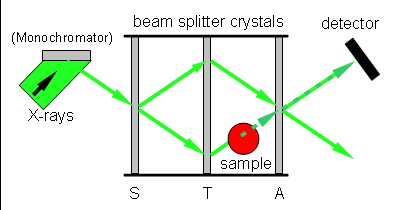
\includegraphics[width=\textwidth]{gfx/Crystal_interferometer.png}
    \caption[Bonse-Hart interferometer.]{A Bonse-Hart crystal
    interferometer\cn. Two coherent beams are created: one is used as a
reference beam, while a sample interacts with the second beam. Imaging is
performed through the
comparison of the interference produced at the third grating by the
reference beam with the sample beam.}
    \label{fig:bonse-hart}
\end{figure}

Again, as for diffraction enhanced techniques, the use of crystals as
optical elements means that only a very narrow bandwidth can be used from a
polychromatic source. Moreover, the three beam splitters should be
manufactured from a single crystal in order to reduce instabilities,
resulting in a limitation on the size of the field of view.

\subsection{Edge illumination}
Edge illumination is not an interferometric technique, although it is
inspired by diffraction enhanced imaging. The basic principle of edge
illumination is the collimation of the X-rays through a narrow aperture,
the resulting beam is then masked by a second aperture whose position is
scanned in a direction perpendicular to the beam: the intensity decreases from a
maximum when the two slits are perfectly aligned as the lateral displacement
of the second mask is increased.
The presence of a sample in the beam introduces refraction, which can be
observed as a displacement of this curve. The same applies to each pixel in
the detector, therefore the period of the source and detector masks have to
be matched so that there is a one-to-one mapping from each aperture in the
source mask to each aperture in the detector mask to each underlying
detector pixel (figure~\ref{fig:edge-illumination}).

\begin{figure}[htb]
    \centering
    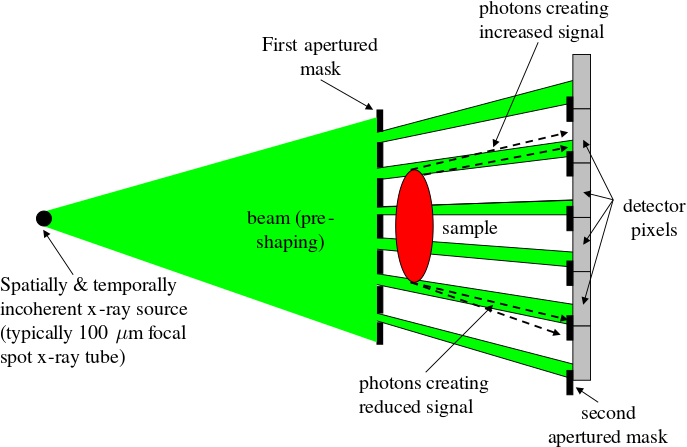
\includegraphics[width=\textwidth]{gfx/edgeillumination.png}
    \caption[Edge illumination.]{An setup for edge illumination\cn. Angular
        deviations of the beams introduced by the object are detected as
        lateral displacements of the fringes of the first mask, analyzed
        through the second mask.}
    \label{fig:edge-illumination}
\end{figure}



This approach does not impose requirements on the spatial or temporal
coherence of the source, and has been successfully run on conventional
laboratory sources.

\subsection{Talbot interferometry}
Talbot interferometry in different configurations is the topic of this
thesis. The Talbot effect will be therefore described in detail.

The Helmoltz equation~\eqref{eq:helmoltz.fourier} provides the solution for
the propagation of a plane wave in a vacuum, where $n \equiv 1$. Plane waves
are solutions

\begin{equation}
    \psi(\omega, \vec{x}) = e^{i\vec{k}\cdot \vec{x}} \qquad \text{with } k^2
    = k_x^2 + k_y^2 + k_z^2 = c^2 \omega^2.
    \label{eq:plane.wave.solution}
\end{equation}

We can then isolate the direction
of propagation $z$, by writing the solution~\eqref{eq:plane.wave.solution} in the form
\begin{equation}
    \psi(\omega, x, y, z) = e^{i(k_x x + k_y y)}e^{iz\sqrt{k^2 - k_x^2 -
    k_y^2}}.
    \label{eq:free.propagation}
\end{equation}
It is then clear that to propagate the plane wave from $z = 0$ to $z = z_0$
it is necessary to multiply by the factor $\exp(iz\sqrt{k^2 - k_x^2 -
k_y^2})$.

Given a general solution to the Helmoltz
equation~\eqref{eq:helmoltz.fourier}, it can be decomposed as a sum of plane
waves through the Fourier transform $\Fxy$ with respect to $x$ and $y$. Each
plane wave then propagates according to
equation~\eqref{eq:free.propagation}. The propagated wave can be then
recovered with the inverse Fourier transform $Fxy^-1$
\begin{equation}
    \psi(\omega, x, y, z_0) = \Fxy^{-1}e^{i z_0 \sqrt{k^2 - k_x^2 -
    k_y^2}}\Fxy    \psi(\omega, x, y, 0).
    \label{eq:full.propagator}
\end{equation}
The paraxial approximation in this context translates to the fact that the
transverse components of the wave vector $\vec{k}$ are much smaller than the
component along the beam path $|k_x|, |k_y| \ll |k_z|$. The square root can
then be approximated to the first order

\begin{equation}
    \sqrt{k^2 - k_x^2 - k_y^2} \approx k - \frac{k_x^2 + k_y^2}{2k}.
    \label{eq:square.root.approximation}
\end{equation}

This yields the final form of the propagator that will be used in the rest
of our analyis
\begin{equation}
    \psi(\omega, x, y, z_0) = e^{i k z_0}\Fxy^{-1}e^{-i z_0\frac{k_x^2 +
    k_y^2}{2k}}\Fxy\psi(\omega, x, y, 0). \label{eq:paraxial.propagator}
\end{equation}

The optical phenomenon discovered in 1836 by Talbot is the observation that
the propagator~\eqref{eq:paraxial.propagator} is equal to one for a periodic
source wave at fixed distances, therefore called \emph{Talbot distances}.

Let's consider for simplicity the one-dimensional case where the
monochromatic field $\psi(\omega, x, z=0)$ is periodic with period $p_1$
along the $x$ direction. 

Then, following the recipe of equation~\eqref{eq:full.propagator}, we need
to calculate the Fourier transform with respect to $x$
\begin{equation*}
    \Fx\psi(\omega, x, 0) = \sum_j \psi_j(\omega)\delta(k_x -
    k_{xj}),
\end{equation*}
in terms of $k_{xj} = 2\pi j/ p_1$ and of the Dirac $\delta$. This is
because the field is periodic with period $p_1$ and only the terms related
to the frequencies $k_{xj}$ will be nonzero after the transform.

By then propagating according to equation~\eqref{eq:paraxial.propagator}

\begin{align}
    \Fx\psi(\omega, x, z_0) &= \exp(ikz_0)\exp(-i z_0\frac{k_x^2}{2k})\sum_j \psi_j(\omega)\delta(k_x -
    k_{xj}) \\
    &= \exp(ikz_0)\exp(-i z_0\frac{k_{xj}^2}{2k})\sum_j \psi_j(\omega)\delta(k_x -
    k_{xj}).
    \label{eq:talbot1}
\end{align}

The effect of the Dirac $\delta$ is to replace $k_x$ with $k_{xj}$, which
means that the propagator will, apart from an irrelevant overall constant phase
factor, be equal to one at distances

\begin{equation}
    \Delta_n = n \frac{p_1^2}{2 \lambda} \qquad n \in
    \mathbb{N}.\label{eq:talbot.distance}
\end{equation}

The source field at $z = 0$ creates a
self-image, exactly replicating its periodic intensity pattern at each
distance $\Delta_n$ downstream, as long as the approximations we introduced
are valid.

This effect can be observed by introducing a grating with absorbing lines in
the beam. However, the resulting intensity will be also reduced by a factor
known as the \emph{duty cycle} of the grating, that is the ratio of the
width of the opening to the pitch of the grating itself. This is not optimal
as it affects exposure times, but it is possible to observe the same effect
by introducing a phase periodicity in the source by letting the X-rays
go through a gratings whose lines change the phase of the radiation by a
factor of $\pi$. A self-image of the grating is then formed with double the
spatial frequency at the Lohmann distances
\begin{equation*}
    D_j = \left(j - \frac{1}{2}\right) \frac{p_1^2}{4 \lambda} \qquad
    j\in\mathbb{N}.
\end{equation*}

The intensity of a monochromatic periodic wave front propagating according to
equation~\eqref{eq:paraxial.propagator} is shown in
figure~\ref{fig:talbotcarpet}.

\begin{figure}[htb]
    \centering
    %% Creator: Matplotlib, PGF backend
%%
%% To include the figure in your LaTeX document, write
%%   \input{<filename>.pgf}
%%
%% Make sure the required packages are loaded in your preamble
%%   \usepackage{pgf}
%%
%% Figures using additional raster images can only be included by \input if
%% they are in the same directory as the main LaTeX file. For loading figures
%% from other directories you can use the `import` package
%%   \usepackage{import}
%% and then include the figures with
%%   \import{<path to file>}{<filename>.pgf}
%%
%% Matplotlib used the following preamble
%%   \usepackage{fontspec}
%%
\begingroup%
\makeatletter%
\begin{pgfpicture}%
\pgfpathrectangle{\pgfpointorigin}{\pgfqpoint{4.600000in}{4.000000in}}%
\pgfusepath{use as bounding box}%
\begin{pgfscope}%
\pgfsetrectcap%
\pgfsetroundjoin%
\definecolor{currentfill}{rgb}{1.000000,1.000000,1.000000}%
\pgfsetfillcolor{currentfill}%
\pgfsetlinewidth{0.000000pt}%
\definecolor{currentstroke}{rgb}{1.000000,1.000000,1.000000}%
\pgfsetstrokecolor{currentstroke}%
\pgfsetdash{}{0pt}%
\pgfpathmoveto{\pgfqpoint{0.000000in}{0.000000in}}%
\pgfpathlineto{\pgfqpoint{4.600000in}{0.000000in}}%
\pgfpathlineto{\pgfqpoint{4.600000in}{4.000000in}}%
\pgfpathlineto{\pgfqpoint{0.000000in}{4.000000in}}%
\pgfpathclose%
\pgfusepath{fill}%
\end{pgfscope}%
\begin{pgfscope}%
\pgfsetrectcap%
\pgfsetroundjoin%
\definecolor{currentfill}{rgb}{1.000000,1.000000,1.000000}%
\pgfsetfillcolor{currentfill}%
\pgfsetlinewidth{0.000000pt}%
\definecolor{currentstroke}{rgb}{0.000000,0.000000,0.000000}%
\pgfsetstrokecolor{currentstroke}%
\pgfsetdash{}{0pt}%
\pgfpathmoveto{\pgfqpoint{0.630833in}{0.516250in}}%
\pgfpathlineto{\pgfqpoint{4.397569in}{0.516250in}}%
\pgfpathlineto{\pgfqpoint{4.397569in}{3.835000in}}%
\pgfpathlineto{\pgfqpoint{0.630833in}{3.835000in}}%
\pgfpathclose%
\pgfusepath{fill}%
\end{pgfscope}%
\begin{pgfscope}%
\pgfpathrectangle{\pgfqpoint{0.630833in}{0.516250in}}{\pgfqpoint{3.766736in}{3.318750in}} %
\pgfusepath{clip}%
\pgftext[at=\pgfqpoint{0.630833in}{0.516250in},left,bottom]{\pgfimage[interpolate=true,width=3.770000in,height=3.323333in]{talbotcarpet-img0.png}}%
\end{pgfscope}%
\begin{pgfscope}%
\pgfsetbuttcap%
\pgfsetroundjoin%
\definecolor{currentfill}{rgb}{0.000000,0.000000,0.000000}%
\pgfsetfillcolor{currentfill}%
\pgfsetlinewidth{1.003750pt}%
\definecolor{currentstroke}{rgb}{0.000000,0.000000,0.000000}%
\pgfsetstrokecolor{currentstroke}%
\pgfsetdash{}{0pt}%
\pgfsys@defobject{currentmarker}{\pgfqpoint{0.000000in}{0.000000in}}{\pgfqpoint{0.000000in}{0.055556in}}{%
\pgfpathmoveto{\pgfqpoint{0.000000in}{0.000000in}}%
\pgfpathlineto{\pgfqpoint{0.000000in}{0.055556in}}%
\pgfusepath{stroke,fill}%
}%
\begin{pgfscope}%
\pgfsys@transformshift{0.631461in}{0.516250in}%
\pgfsys@useobject{currentmarker}{}%
\end{pgfscope}%
\end{pgfscope}%
\begin{pgfscope}%
\pgftext[left,bottom,x=0.594030in,y=0.342000in,rotate=0.000000]{{\rmfamily\fontsize{11.000000}{13.200000}\selectfont 0}}
%
\end{pgfscope}%
\begin{pgfscope}%
\pgfsetbuttcap%
\pgfsetroundjoin%
\definecolor{currentfill}{rgb}{0.000000,0.000000,0.000000}%
\pgfsetfillcolor{currentfill}%
\pgfsetlinewidth{1.003750pt}%
\definecolor{currentstroke}{rgb}{0.000000,0.000000,0.000000}%
\pgfsetstrokecolor{currentstroke}%
\pgfsetdash{}{0pt}%
\pgfsys@defobject{currentmarker}{\pgfqpoint{0.000000in}{0.000000in}}{\pgfqpoint{0.000000in}{0.055556in}}{%
\pgfpathmoveto{\pgfqpoint{0.000000in}{0.000000in}}%
\pgfpathlineto{\pgfqpoint{0.000000in}{0.055556in}}%
\pgfusepath{stroke,fill}%
}%
\begin{pgfscope}%
\pgfsys@transformshift{1.384683in}{0.516250in}%
\pgfsys@useobject{currentmarker}{}%
\end{pgfscope}%
\end{pgfscope}%
\begin{pgfscope}%
\pgftext[left,bottom,x=1.347252in,y=0.345208in,rotate=0.000000]{{\rmfamily\fontsize{11.000000}{13.200000}\selectfont 1}}
%
\end{pgfscope}%
\begin{pgfscope}%
\pgfsetbuttcap%
\pgfsetroundjoin%
\definecolor{currentfill}{rgb}{0.000000,0.000000,0.000000}%
\pgfsetfillcolor{currentfill}%
\pgfsetlinewidth{1.003750pt}%
\definecolor{currentstroke}{rgb}{0.000000,0.000000,0.000000}%
\pgfsetstrokecolor{currentstroke}%
\pgfsetdash{}{0pt}%
\pgfsys@defobject{currentmarker}{\pgfqpoint{0.000000in}{0.000000in}}{\pgfqpoint{0.000000in}{0.055556in}}{%
\pgfpathmoveto{\pgfqpoint{0.000000in}{0.000000in}}%
\pgfpathlineto{\pgfqpoint{0.000000in}{0.055556in}}%
\pgfusepath{stroke,fill}%
}%
\begin{pgfscope}%
\pgfsys@transformshift{2.137904in}{0.516250in}%
\pgfsys@useobject{currentmarker}{}%
\end{pgfscope}%
\end{pgfscope}%
\begin{pgfscope}%
\pgftext[left,bottom,x=2.042265in,y=0.342000in,rotate=0.000000]{{\rmfamily\fontsize{11.000000}{13.200000}\selectfont 1.5}}
%
\end{pgfscope}%
\begin{pgfscope}%
\pgfsetbuttcap%
\pgfsetroundjoin%
\definecolor{currentfill}{rgb}{0.000000,0.000000,0.000000}%
\pgfsetfillcolor{currentfill}%
\pgfsetlinewidth{1.003750pt}%
\definecolor{currentstroke}{rgb}{0.000000,0.000000,0.000000}%
\pgfsetstrokecolor{currentstroke}%
\pgfsetdash{}{0pt}%
\pgfsys@defobject{currentmarker}{\pgfqpoint{0.000000in}{0.000000in}}{\pgfqpoint{0.000000in}{0.055556in}}{%
\pgfpathmoveto{\pgfqpoint{0.000000in}{0.000000in}}%
\pgfpathlineto{\pgfqpoint{0.000000in}{0.055556in}}%
\pgfusepath{stroke,fill}%
}%
\begin{pgfscope}%
\pgfsys@transformshift{2.891126in}{0.516250in}%
\pgfsys@useobject{currentmarker}{}%
\end{pgfscope}%
\end{pgfscope}%
\begin{pgfscope}%
\pgftext[left,bottom,x=2.853695in,y=0.345208in,rotate=0.000000]{{\rmfamily\fontsize{11.000000}{13.200000}\selectfont 2}}
%
\end{pgfscope}%
\begin{pgfscope}%
\pgfsetbuttcap%
\pgfsetroundjoin%
\definecolor{currentfill}{rgb}{0.000000,0.000000,0.000000}%
\pgfsetfillcolor{currentfill}%
\pgfsetlinewidth{1.003750pt}%
\definecolor{currentstroke}{rgb}{0.000000,0.000000,0.000000}%
\pgfsetstrokecolor{currentstroke}%
\pgfsetdash{}{0pt}%
\pgfsys@defobject{currentmarker}{\pgfqpoint{0.000000in}{0.000000in}}{\pgfqpoint{0.000000in}{0.055556in}}{%
\pgfpathmoveto{\pgfqpoint{0.000000in}{0.000000in}}%
\pgfpathlineto{\pgfqpoint{0.000000in}{0.055556in}}%
\pgfusepath{stroke,fill}%
}%
\begin{pgfscope}%
\pgfsys@transformshift{3.644348in}{0.516250in}%
\pgfsys@useobject{currentmarker}{}%
\end{pgfscope}%
\end{pgfscope}%
\begin{pgfscope}%
\pgftext[left,bottom,x=3.548709in,y=0.342000in,rotate=0.000000]{{\rmfamily\fontsize{11.000000}{13.200000}\selectfont 2.5}}
%
\end{pgfscope}%
\begin{pgfscope}%
\pgfsetbuttcap%
\pgfsetroundjoin%
\definecolor{currentfill}{rgb}{0.000000,0.000000,0.000000}%
\pgfsetfillcolor{currentfill}%
\pgfsetlinewidth{1.003750pt}%
\definecolor{currentstroke}{rgb}{0.000000,0.000000,0.000000}%
\pgfsetstrokecolor{currentstroke}%
\pgfsetdash{}{0pt}%
\pgfsys@defobject{currentmarker}{\pgfqpoint{0.000000in}{0.000000in}}{\pgfqpoint{0.000000in}{0.055556in}}{%
\pgfpathmoveto{\pgfqpoint{0.000000in}{0.000000in}}%
\pgfpathlineto{\pgfqpoint{0.000000in}{0.055556in}}%
\pgfusepath{stroke,fill}%
}%
\begin{pgfscope}%
\pgfsys@transformshift{4.397569in}{0.516250in}%
\pgfsys@useobject{currentmarker}{}%
\end{pgfscope}%
\end{pgfscope}%
\begin{pgfscope}%
\pgftext[left,bottom,x=4.360139in,y=0.342000in,rotate=0.000000]{{\rmfamily\fontsize{11.000000}{13.200000}\selectfont 3}}
%
\end{pgfscope}%
\begin{pgfscope}%
\pgftext[left,bottom,x=1.827083in,y=0.165000in,rotate=0.000000]{{\rmfamily\fontsize{11.000000}{13.200000}\selectfont distanze di Lohmann}}
%
\end{pgfscope}%
\begin{pgfscope}%
\pgfsetbuttcap%
\pgfsetroundjoin%
\definecolor{currentfill}{rgb}{0.000000,0.000000,0.000000}%
\pgfsetfillcolor{currentfill}%
\pgfsetlinewidth{1.003750pt}%
\definecolor{currentstroke}{rgb}{0.000000,0.000000,0.000000}%
\pgfsetstrokecolor{currentstroke}%
\pgfsetdash{}{0pt}%
\pgfsys@defobject{currentmarker}{\pgfqpoint{0.000000in}{0.000000in}}{\pgfqpoint{0.055556in}{0.000000in}}{%
\pgfpathmoveto{\pgfqpoint{0.000000in}{0.000000in}}%
\pgfpathlineto{\pgfqpoint{0.055556in}{0.000000in}}%
\pgfusepath{stroke,fill}%
}%
\begin{pgfscope}%
\pgfsys@transformshift{0.630833in}{0.517633in}%
\pgfsys@useobject{currentmarker}{}%
\end{pgfscope}%
\end{pgfscope}%
\begin{pgfscope}%
\pgftext[left,bottom,x=0.370111in,y=0.465230in,rotate=0.000000]{{\rmfamily\fontsize{11.000000}{13.200000}\selectfont 0.0}}
%
\end{pgfscope}%
\begin{pgfscope}%
\pgfsetbuttcap%
\pgfsetroundjoin%
\definecolor{currentfill}{rgb}{0.000000,0.000000,0.000000}%
\pgfsetfillcolor{currentfill}%
\pgfsetlinewidth{1.003750pt}%
\definecolor{currentstroke}{rgb}{0.000000,0.000000,0.000000}%
\pgfsetstrokecolor{currentstroke}%
\pgfsetdash{}{0pt}%
\pgfsys@defobject{currentmarker}{\pgfqpoint{0.000000in}{0.000000in}}{\pgfqpoint{0.055556in}{0.000000in}}{%
\pgfpathmoveto{\pgfqpoint{0.000000in}{0.000000in}}%
\pgfpathlineto{\pgfqpoint{0.055556in}{0.000000in}}%
\pgfusepath{stroke,fill}%
}%
\begin{pgfscope}%
\pgfsys@transformshift{0.630833in}{1.070758in}%
\pgfsys@useobject{currentmarker}{}%
\end{pgfscope}%
\end{pgfscope}%
\begin{pgfscope}%
\pgftext[left,bottom,x=0.370111in,y=1.018355in,rotate=0.000000]{{\rmfamily\fontsize{11.000000}{13.200000}\selectfont 0.5}}
%
\end{pgfscope}%
\begin{pgfscope}%
\pgfsetbuttcap%
\pgfsetroundjoin%
\definecolor{currentfill}{rgb}{0.000000,0.000000,0.000000}%
\pgfsetfillcolor{currentfill}%
\pgfsetlinewidth{1.003750pt}%
\definecolor{currentstroke}{rgb}{0.000000,0.000000,0.000000}%
\pgfsetstrokecolor{currentstroke}%
\pgfsetdash{}{0pt}%
\pgfsys@defobject{currentmarker}{\pgfqpoint{0.000000in}{0.000000in}}{\pgfqpoint{0.055556in}{0.000000in}}{%
\pgfpathmoveto{\pgfqpoint{0.000000in}{0.000000in}}%
\pgfpathlineto{\pgfqpoint{0.055556in}{0.000000in}}%
\pgfusepath{stroke,fill}%
}%
\begin{pgfscope}%
\pgfsys@transformshift{0.630833in}{1.623883in}%
\pgfsys@useobject{currentmarker}{}%
\end{pgfscope}%
\end{pgfscope}%
\begin{pgfscope}%
\pgftext[left,bottom,x=0.370111in,y=1.571480in,rotate=0.000000]{{\rmfamily\fontsize{11.000000}{13.200000}\selectfont 1.0}}
%
\end{pgfscope}%
\begin{pgfscope}%
\pgfsetbuttcap%
\pgfsetroundjoin%
\definecolor{currentfill}{rgb}{0.000000,0.000000,0.000000}%
\pgfsetfillcolor{currentfill}%
\pgfsetlinewidth{1.003750pt}%
\definecolor{currentstroke}{rgb}{0.000000,0.000000,0.000000}%
\pgfsetstrokecolor{currentstroke}%
\pgfsetdash{}{0pt}%
\pgfsys@defobject{currentmarker}{\pgfqpoint{0.000000in}{0.000000in}}{\pgfqpoint{0.055556in}{0.000000in}}{%
\pgfpathmoveto{\pgfqpoint{0.000000in}{0.000000in}}%
\pgfpathlineto{\pgfqpoint{0.055556in}{0.000000in}}%
\pgfusepath{stroke,fill}%
}%
\begin{pgfscope}%
\pgfsys@transformshift{0.630833in}{2.177008in}%
\pgfsys@useobject{currentmarker}{}%
\end{pgfscope}%
\end{pgfscope}%
\begin{pgfscope}%
\pgftext[left,bottom,x=0.370111in,y=2.124605in,rotate=0.000000]{{\rmfamily\fontsize{11.000000}{13.200000}\selectfont 1.5}}
%
\end{pgfscope}%
\begin{pgfscope}%
\pgfsetbuttcap%
\pgfsetroundjoin%
\definecolor{currentfill}{rgb}{0.000000,0.000000,0.000000}%
\pgfsetfillcolor{currentfill}%
\pgfsetlinewidth{1.003750pt}%
\definecolor{currentstroke}{rgb}{0.000000,0.000000,0.000000}%
\pgfsetstrokecolor{currentstroke}%
\pgfsetdash{}{0pt}%
\pgfsys@defobject{currentmarker}{\pgfqpoint{0.000000in}{0.000000in}}{\pgfqpoint{0.055556in}{0.000000in}}{%
\pgfpathmoveto{\pgfqpoint{0.000000in}{0.000000in}}%
\pgfpathlineto{\pgfqpoint{0.055556in}{0.000000in}}%
\pgfusepath{stroke,fill}%
}%
\begin{pgfscope}%
\pgfsys@transformshift{0.630833in}{2.730133in}%
\pgfsys@useobject{currentmarker}{}%
\end{pgfscope}%
\end{pgfscope}%
\begin{pgfscope}%
\pgftext[left,bottom,x=0.370111in,y=2.677730in,rotate=0.000000]{{\rmfamily\fontsize{11.000000}{13.200000}\selectfont 2.0}}
%
\end{pgfscope}%
\begin{pgfscope}%
\pgfsetbuttcap%
\pgfsetroundjoin%
\definecolor{currentfill}{rgb}{0.000000,0.000000,0.000000}%
\pgfsetfillcolor{currentfill}%
\pgfsetlinewidth{1.003750pt}%
\definecolor{currentstroke}{rgb}{0.000000,0.000000,0.000000}%
\pgfsetstrokecolor{currentstroke}%
\pgfsetdash{}{0pt}%
\pgfsys@defobject{currentmarker}{\pgfqpoint{0.000000in}{0.000000in}}{\pgfqpoint{0.055556in}{0.000000in}}{%
\pgfpathmoveto{\pgfqpoint{0.000000in}{0.000000in}}%
\pgfpathlineto{\pgfqpoint{0.055556in}{0.000000in}}%
\pgfusepath{stroke,fill}%
}%
\begin{pgfscope}%
\pgfsys@transformshift{0.630833in}{3.283258in}%
\pgfsys@useobject{currentmarker}{}%
\end{pgfscope}%
\end{pgfscope}%
\begin{pgfscope}%
\pgftext[left,bottom,x=0.370111in,y=3.230855in,rotate=0.000000]{{\rmfamily\fontsize{11.000000}{13.200000}\selectfont 2.5}}
%
\end{pgfscope}%
\begin{pgfscope}%
\pgftext[left,bottom,x=0.300667in,y=1.742156in,rotate=90.000000]{{\rmfamily\fontsize{11.000000}{13.200000}\selectfont periodi di \(\displaystyle G_1\)}}
%
\end{pgfscope}%
\begin{pgfscope}%
\pgfsetrectcap%
\pgfsetroundjoin%
\pgfsetlinewidth{1.003750pt}%
\definecolor{currentstroke}{rgb}{0.000000,0.000000,0.000000}%
\pgfsetstrokecolor{currentstroke}%
\pgfsetdash{}{0pt}%
\pgfpathmoveto{\pgfqpoint{0.630833in}{3.835000in}}%
\pgfpathlineto{\pgfqpoint{4.397569in}{3.835000in}}%
\pgfusepath{stroke}%
\end{pgfscope}%
\begin{pgfscope}%
\pgfsetrectcap%
\pgfsetroundjoin%
\pgfsetlinewidth{1.003750pt}%
\definecolor{currentstroke}{rgb}{0.000000,0.000000,0.000000}%
\pgfsetstrokecolor{currentstroke}%
\pgfsetdash{}{0pt}%
\pgfpathmoveto{\pgfqpoint{4.397569in}{0.516250in}}%
\pgfpathlineto{\pgfqpoint{4.397569in}{3.835000in}}%
\pgfusepath{stroke}%
\end{pgfscope}%
\begin{pgfscope}%
\pgfsetrectcap%
\pgfsetroundjoin%
\pgfsetlinewidth{1.003750pt}%
\definecolor{currentstroke}{rgb}{0.000000,0.000000,0.000000}%
\pgfsetstrokecolor{currentstroke}%
\pgfsetdash{}{0pt}%
\pgfpathmoveto{\pgfqpoint{0.630833in}{0.516250in}}%
\pgfpathlineto{\pgfqpoint{4.397569in}{0.516250in}}%
\pgfusepath{stroke}%
\end{pgfscope}%
\begin{pgfscope}%
\pgfsetrectcap%
\pgfsetroundjoin%
\pgfsetlinewidth{1.003750pt}%
\definecolor{currentstroke}{rgb}{0.000000,0.000000,0.000000}%
\pgfsetstrokecolor{currentstroke}%
\pgfsetdash{}{0pt}%
\pgfpathmoveto{\pgfqpoint{0.630833in}{0.516250in}}%
\pgfpathlineto{\pgfqpoint{0.630833in}{3.835000in}}%
\pgfusepath{stroke}%
\end{pgfscope}%
\end{pgfpicture}%
\makeatother%
\endgroup%

    \caption[Talbot carpet.]{Simulation of the \emph{Talbot carpet},
    that is the propagation of a wave front with a phase periodicity
    introduced by a grating \G1.
    Interference fringes are created at the Lohmann distances with half the
period of the grating \G1.}
    \label{fig:talbotcarpet}
\end{figure}

\section{Talbot-Lau interferometry}
\subsection{Image generation and analysis}
The fundamental principle of Talbot interferometry lies in the self-imaging
property of a periodic wave front as described in the previous section. A
sample can then be introduced in the beam, resulting in a reshaping of the
interference pattern.

Specifically, refraction of the X-ray beam produces a lateral displacement
of the interference fringes. The direction of propagation of a plane wave
\begin{equation}
    e^{-i \vec{k} \cdot \vec{x}} = e^{-i\varphi(x)}
    \label{eq:plane.wave}
\end{equation}
is determined by the unit vector
\begin{equation}
    \vec{n} = -\frac{1}{k} \nabla\varphi.
    \label{eq:plane.wave.direction}
\end{equation}
Therefore, the angular deviation of the beam along the axis $x$ perpendicular to
the direction of propagation and to the direction of the grating lines is
\begin{equation}
        \alpha = -\frac{1}{k} \partial_x\varphi.\label{eq:refraction.angle}
\end{equation}
This deviation would be measurable as a lateral displacement of the
interference fringes of the Talbot self-image of the grating \G1, with the
\emph{caveat} that this interference pattern has a pitch of the order of
few micrometers and is therefore not resolved by detectors with a pixel size
that is one or two orders of magnitude larger, although some applications
exist on synchrotron sources for a limited field of view\cn.

For this reason, a second grating \G2 with absorbing lines is placed at the
location where the self-image of \G1 is created with the same period of the
interference pattern. This grating is then laterally displaced in the $x$
direction: when the grating lines of \G2
match the bright lines of the interference pattern, the intensity recorded
by the underlying detector pixel reaches a minimum, whereas when the
absorbing lines are superimposed to the dark lines the radiation is able to
go through and a maximum intensity is recorded. Sliding the grating \G2
along the rectangular interference pattern of \G1 corresponds to recording
the convolution of the two signals. The result is a triangular signal, known
as the \emph{phase stepping curve}.

A triangular phase stepping curve is the result of the convolution of the
two rectangular shapes of the grating transmissions. However, a finite
source size also affects the shape of the curve by convolving the signal
with the image of the source. The result is calculated in detail in\cn, we
are here interested in the result pictured in
figure~\ref{fig:phase.stepping.sinusoidal}: the curve is well approximated by a
sinusoid
\begin{equation*}
    s(x) = a_0 + a_1 \cos \left(\frac{2 \pi}{p_2} x + \theta\right).
\end{equation*}

\begin{figure}[htb]
    \centering
    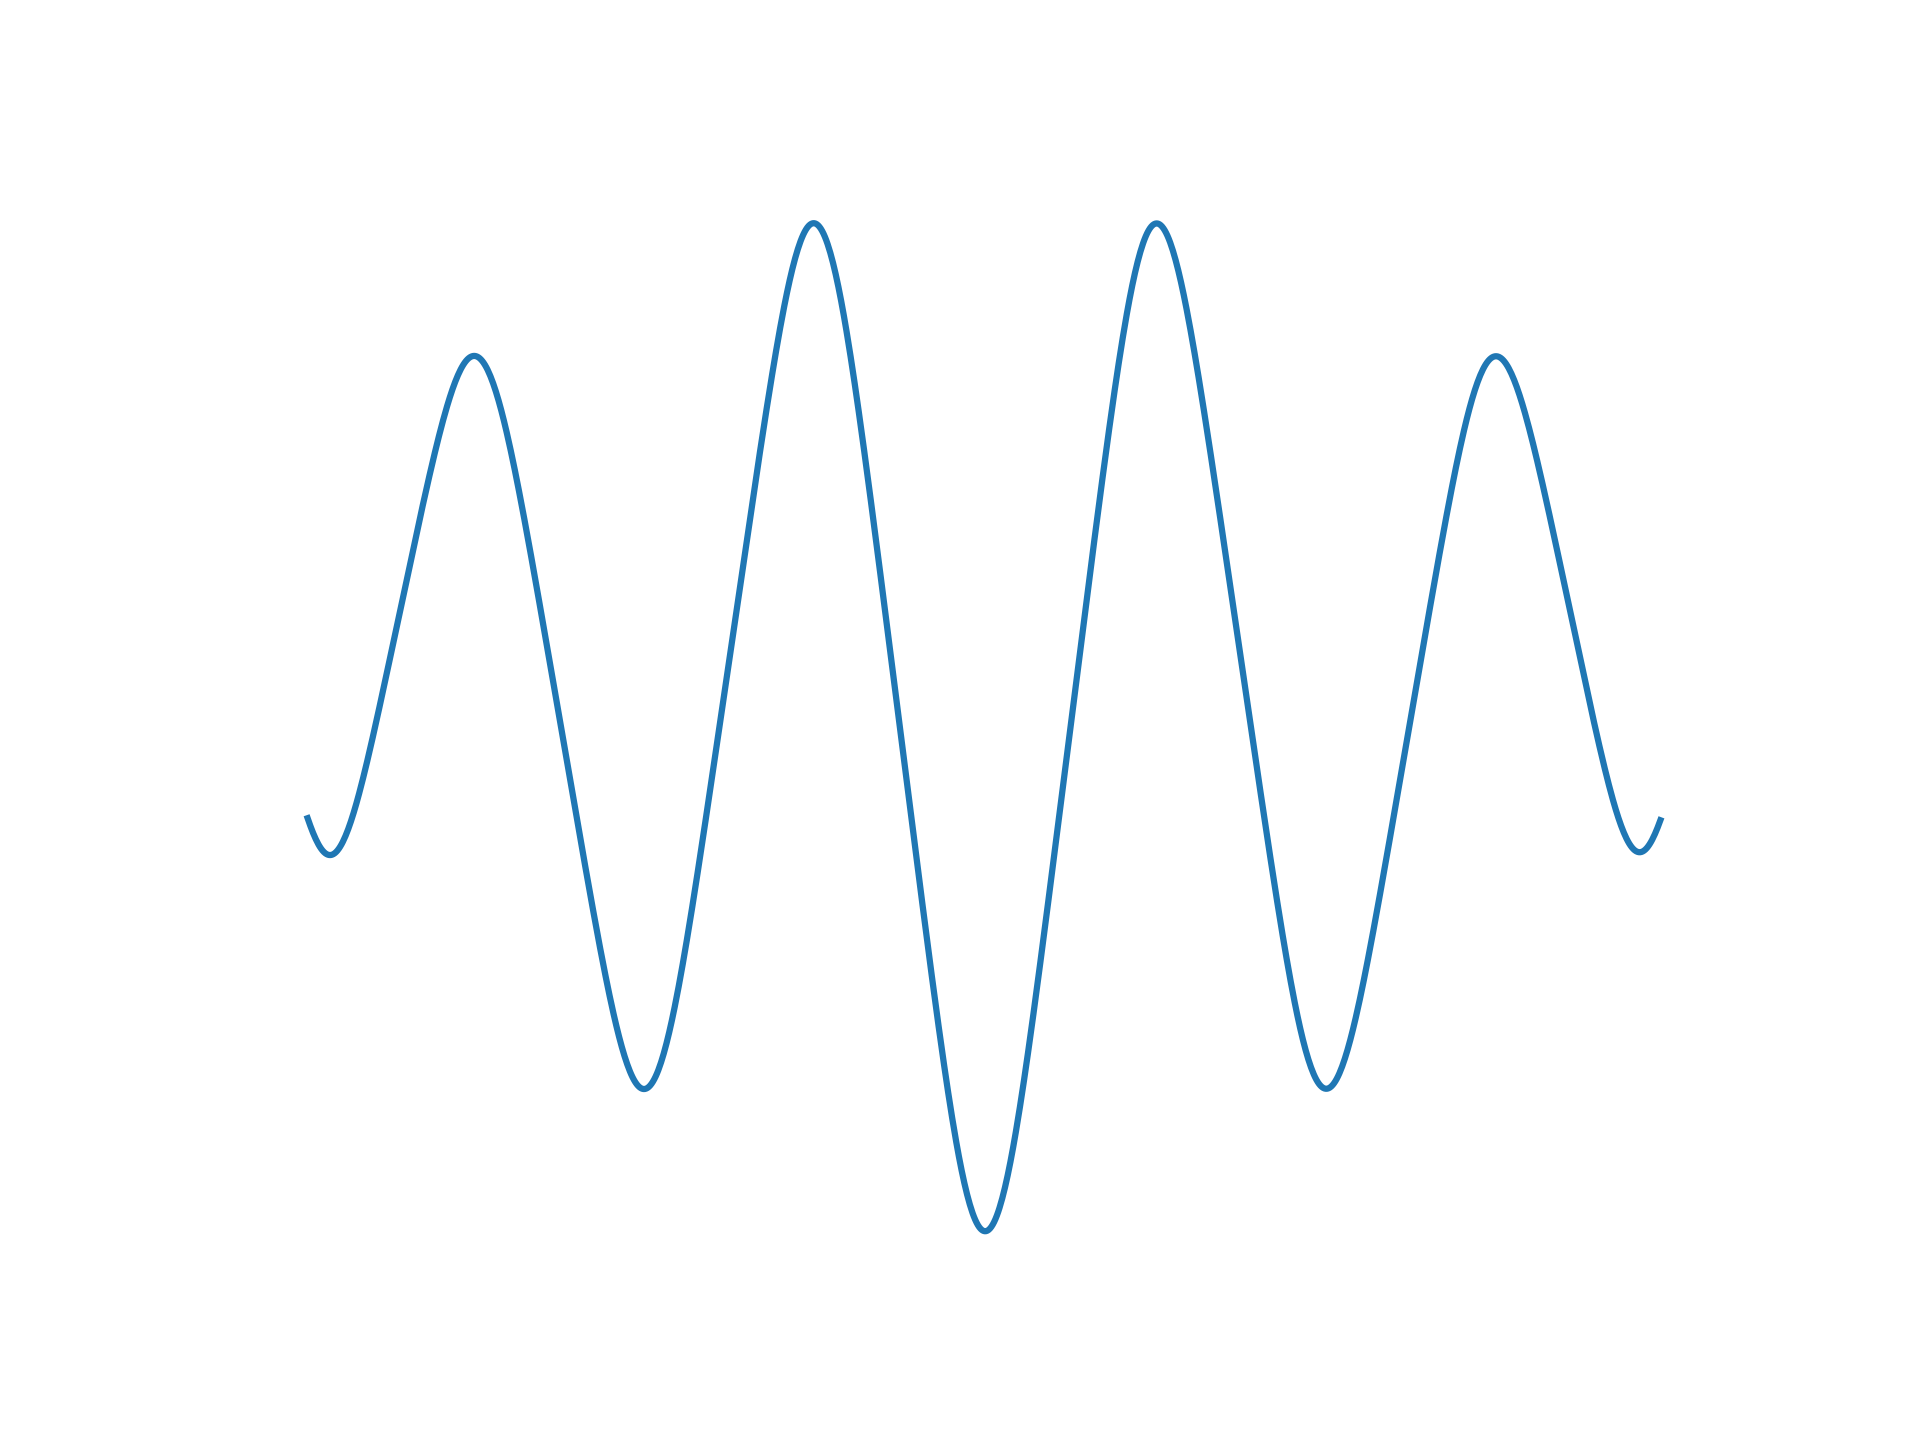
\includegraphics[width=\textwidth]{gfx/sinusoidal-phase-stepping/sinusoidal-phase-stepping.png}
    \caption[Convolution of two rectangular and a gaussian signal.]{The
        plotted function is the result of the convolution of two rectangular
        signals, representing the self image of the phase grating \G1 and the
        transmission function of the analyzer grating \G2, and a gaussian
    signal representing a finite source profile.}
    \label{fig:phase.stepping.sinusoidal}
\end{figure}


A number of \emph{phase steps} are then recorded for different displacements
$x$ of \G2 and the three parameters $a_0$, $a_1$ and $\theta$ are determined
with a linear fit performed by means of a discrete fast Fourier transform~\cite{FFTEquivalence}.

A reference, or \emph{flat}, curve is then compared to the curve observed
with the sample in the beam, or \emph{sample} curve

\begin{align}
    s_f(x) &= a_{0,f} + a_{1,f} \cos\left(\frac{2 \pi}{p_2} x + \theta_{f}\right)\\
    s_s(x) &= a_{0,s} + a_{1,s} \cos\left(\frac{2 \pi}{p_2} x +
    \theta_{s}\right).
    \label{eq:flat}
\end{align}

\begin{figure}[htb]
    \centering
    \input{gfx/phase_stepping.eepic}
    \caption[Phase stepping curve.]{The analyzer grating \G{2} scans the
    interference pattern by sliding on a direction perpendicular to the
    fringes. An intensity curve is recorded on each pixel, allowing the
    retrieval of three parameters: the average $a_0$, the amplitude $a_1$
and the phase $\theta$.}
    \label{fig:phase.stepping}
\end{figure}

Three complementary signals can be determined by these parameters
(figure~\ref{fig:phase.stepping}):
\begin{description}
    \item[transmission,] given by the ratio $A = a_{0,c} / a_{0,f}$, is the
        intensity of the transmitted radiation, as in conventional
        radiography, related to the Beer-Lambert
        law~\eqref{eq:beer-lambert}.
    \item[differential phase,] or the difference $P = \theta_{c} -
        \theta_f$, depending on the lateral displacement of the interference
        fringes given by
        $\alpha$~\eqref{eq:refraction.angle} at the
        $j$th Lohmann distance according to
        \begin{equation*}
            P = 2\pi \frac{D_j}{p_2}\alpha.
        \end{equation*}
        It is a differential phase signal because it is proportional to the
        derivative of the phase displacement introduced by the sample.
    \item[visibility reduction,] also known as 
        \emph{scattering} or \emph{dark field} contrast. The
        \emph{visibility} of the curve is the parameter
        $v = 2a_1 / a_0$. The ratio
        \begin{equation*}
            B = \frac{v_c}{v_f} =
            \frac{a_{1,c}}{a_{0,c}}\frac{a_{0,f}}{a_{1,f}}
        \end{equation*}
        is influenced by inhomogeneities of the sample on a scale smaller
        than a detector pixel\cn.
\end{description}

\subsection{Spatial and temporal coherence}
Talbot interferometry is compatible with laboratory sources with a wide
\emph{bremsstrahlung} spectrum. It has been shown\cn that the spectral
acceptance at the $j$th Lohmann distance is
\begin{equation}
    \frac{\Delta \lambda}{\lambda} = \frac{1}{2j - 1}.\label{eq:acceptance}
\end{equation}
Our experiments are designed for sources with a high voltage and a wide
spectrum, typical of security, medical and material science applications.
Therefore, given the inverse proportionality between Lohmann order
and spectral acceptance, our interferometers operate at the first order.

Spatial coherence is more critical for the formation of the self-image of
the grating \G1, in the direction perpendicular to the grating lines --- since no
interference is observed along the grating lines there
is no coherence requirement in that direction.

Let's consider two point sources producing an interference pattern at a
distance $D_j$ from \G1, if the separation between the two points is
$\epsilon$, the two patterns will be shifted by $\epsilon D_j / \ell$: if
this distance is such that the bright lines of one pattern
overlap with the dark lines of the second pattern, the interference will
disappear. We can therefore establish a maximum source width for the
interference effect to occur as
\begin{equation}
    s < \frac{p_2\ell}{2D_j}.
    \label{eq:source.size}
\end{equation}

Synchrotron sources can achieve the required coherence without additional
optical elements, but laboratory sources have a much larger focal spot. If
for instance $\ell = \SI{1}{\meter}$, $D_j = \SI{10}{\centi\meter}$, then
the source has to be smaller than \SI{5}{\micro\meter} which is only
achievable with a microfocus source. This source would provide a very small
amount of radiation for imaging, requiring long exposure times.

This problem can be overcome by placing an additional grating \G0 in front
of the source. The \G0 grating creates an array of individually coherent but
mutually incoherent sources, whose interference patterns superimpose if the
geometrical constraint
\begin{equation}
    p_0 = p_2 \frac{\ell}{D_j}\label{eq:p0}
\end{equation}
is met.

Laboratory sources on a compact setup which are the goal of our experiments
also introduce a significant geometrical magnification. The equations above
all assume a plane wave geometry, but this can be easily adapted for a
spherical wave front according to~\cite{Engelhardt2008}.

The Lohmann distances are rescaled according to
\begin{equation*}
    D_j^\prime = D_j \frac{1}{1 - \dfrac{D_j}{\ell}}.
\end{equation*}

The period of the grating $p_2$ is rescaled by the same factor
\begin{equation}
    p_2^\prime = p_2 \frac{1}{1 -
        \dfrac{D_j}{\ell}}.\label{eq:magnification}
\end{equation}

As a conclusion, we opt for Talbot-Lau interferometry as our tool since it
provides three different and complementary sources of contrast and it is
possible to install it on laboratory sources with a wide spectrum. The
Talbot effect is the key to providing an interference pattern at a
macroscopic distance from the optical elements composing the interferometer
so that there is space to insert a sample and compare the interference
pattern with and without sample to determine its properties.
